\documentclass{article}

\usepackage[utf8]{inputenc}
\usepackage[T1]{fontenc}
\usepackage[norsk,english]{babel}   %Norsk først så engelsk, så engelsk blir prioritert
\usepackage{graphicx}
\usepackage{amsmath}        %For å kunne skrive matte
\usepackage{listings}       %For å kunne skrive inn kode med fin formatering
\usepackage{multicol}       %Importerer pakken for multikolonner til teksten
\usepackage[margin=2.54cm]{geometry}    %Definerer hva bredden til teksten er
\usepackage{wrapfig}    %Importerer pakken for å ha bildene i teksten
\usepackage[font = small]{caption}

%Definerer hyperlinker og dens farger
\usepackage{hyperref}
\hypersetup{
    colorlinks,
    citecolor=blue,
    filecolor=black,
    linkcolor=blue,
    urlcolor=blue
}

%-----------------------------------

%Definerer farger til kodeeksemplene i PDF-en
\usepackage{color}

\definecolor{codegreen}{rgb}{0,0.6,0}
\definecolor{codegray}{rgb}{0.5,0.5,0.5}
\definecolor{codepurple}{rgb}{0.58,0,0.82}
\definecolor{backcolour}{rgb}{0.95,0.95,0.92}

\lstdefinestyle{mystyle}{
    backgroundcolor=\color{backcolour},
    commentstyle=\color{codegreen},
    keywordstyle=\color{magenta},
    numberstyle=\tiny\color{codegray},
    stringstyle=\color{codepurple},
    basicstyle=\footnotesize,
    breakatwhitespace=false,
    breaklines=true,
    captionpos=b,
    keepspaces=true,
    numbers=left,
    numbersep=5pt,
    showspaces=false,
    showstringspaces=false,
    showtabs=false,
    tabsize=2
}

\lstset{style=mystyle}

%------------------------------------

\setlength{\parindent}{0pt} %Ingen indent automaisk for nye linjer
%\setlength{\columnsep}{2mm} %Column separation - til multicolumn

%\setlength{\arrayrulewidth}{1mm}   %Hvilken tykkelse tabellene skal ha
\setlength{\tabcolsep}{2mm}     %Lengden mellom hver kolonne
\renewcommand{\arraystretch}{1.5}   %Hvor stor avstand det skal være mellom radene

\iffalse    %midlertidig endre bredden på teksten
If you want to change this temporarily, you can write:
\savegeometry{mydefaultgeometry}
\newgeometry{margin=3in}
And then later you can call:
\loadgeometry{mydefaultgeometry}
\fi

%for å fjerne overskriften "refrences" som kommer automatisk når man bruker bibtex
\usepackage{etoolbox}
\patchcmd{\thebibliography}{\section*{\refname}}{}{}{}

%----------------------------------------------------------------------------------------

\begin{document}

\addtocounter{page}{0}

\title{Project 3 \\
      \large For the course FYS3150}
\date{\today \\
    \vspace{1mm}
    \large Week 40 - 43}

\author{Erik Grammeltvedt, Erlend Tiberg North and Alexandra Jahr Kolstad}

\maketitle

%\newpage

%------------Her starter skrivingen-----------------------------------------

%\begin{multicols}{2}


%-------------------- Abstract -------------------------------
\vspace{1cm}


\begin{center}

{\Large\textbf{Abstract}} \label{sec:Abstract}

\end{center}


In this scientific study we will compute an integral with different numerical methods of integration to approximate the ground state correlation energy between two electrons in a helium atom. Our integral is given by equation (\ref{eq:integral}). The integral has the analytical answer $\frac{5 \pi^2}{16^2} \approx 0.192765710958777$. The main interest and the goal of this study is to look at how the methods compare with different amount of mesh points and integration limits. The numerical integration methods we will use are Gauss-Legendre quadrature, Gauss-Laguerre quadrature, brute force Monte Carlo, spherical Monte Carlo, and spherical Monte Carlo with parallelization. The study was a success and proved Monte Carlo to be the fastest and most accurate method. In fact, the improved spherical Monte Carlo was $3572\times$ faster than Gauss-Laguerre in achieving an error $|\varepsilon|<0.001$. Being based on big data, it required many more sampling points. However, as it did not manually calculate the integral, it was astronomically much more efficient. \\


\newpage

%------------------- Table of contents -----------------------

\vspace{1cm}

\tableofcontents

\vspace{1cm}

%-------------------- Introduction ------------------------------
\vspace{1cm}

\section{Introduction} \label{sec:Introduction}

Numerical integration methods can be used to numerically solve this integral. For instance Gaussian quadrature uses orthogonal polynomials to compute weights and then Taylor series to approximate the integral. The Gauss-Legendre method implements the theory without further thought to effectiveness. Therefore this method is called brute force Gauss-Legendre, and uses the cartesian coordinate system. An improved Gaussian quadrature rule would be based on a set of polynomials fitting to the integral. In this case, spherical coordinates. This leads to an increase in accuracy, but by that same token, can lead to a longer run-time. The Monte Carlo method is based on probability distribution functions (PDF) to randomly choose numbers in a given interval, and approximate the integral with this set of numbers and given integration points. Each run through Monte Carlo generates a new set of random numbers, which ensures the accuracy. A higher number of integration points will give a better approximation. Monte Carlo integration depends on the PDF chosen, which is specific for different applications. For instance in this study we use the Mersenne Twister 19937 64 bit, a widely known pseudorandom number generator, to generate random numbers in the distribution of the PDF. Therefore, the choice of PDF affect the results, because the distribution of the numbers varies. In this study we implement the uniform distribution for all of the Monte Carlo methods. Monte Carlo also varies with the choice of coordinate system, as the Gaussian quadrature rules do. The brute force Monte Carlo method is based on cartesian coordinates, while the improved Monte Carlo method is based on spherical coordinates. Lastly in this study, we implement parallelization on the improved spherical Monte Carlo method to investigate if there is any change in computation time. These two methods are based on the same Monte Carlo integration and should therefore produce similar results. \\

The integral we are evaluating comes from the solution of Schrödinger's equation for a simplified case of determining the ground state correlation energy between two electrons in a helium atom.

\begin{equation} \label{eq:integral}
    \left\langle \frac{1}{| \vec{r_1} - \vec{r_2} |} \right\rangle = \int_{-\infty} ^\infty d \vec{r_1} d \vec{r_2} \hspace{1mm} e^{- 2 \alpha (r_1 + r_2)} \hspace{1mm} \frac{1}{| \vec{r_1} - \vec{r_2} |}
\end{equation} \\

The integral is not properly normalized. However, that is not important for the study. If you are interested in how the integral is found, see \cite{task}.\\

Our aim is to approximate this integral using two types of Gaussian quadrature, and some variations of Monte Carlo. We have created a code that evaluates the integral using each method and compares them. Alongside the actual value we get the absolute error, $|\varepsilon|$, and time used. Using this we present our data and show that Monte Carlo massively outperforms the Gaussian quadrature rules, especially so after implementing parallelization for the spherical Monte Carlo method. \\

The study will go through the theory and methods behind our study and following that we will present our results and discuss them. Lastly we have a conclusion to briefly summarise our findings. Other findings which we deemed to not be as important are found in the appendix, for instance calculations for proving spherical Monte Carlo method's superiorness over improved Guassian quadrature (\ref{MC>GQ}). Sources of different academic materials we used are given in references. \\


%-------------------- Theory ------------------------------------
\vspace{1cm}

\section{Theory} \label{sec:Theory}

\subsection{Theory of Gaussian quadrature and the Gauss-Legendre method}

The Gauss-Legendre method is based on the more general Gaussian quadrature rule which uses Taylor series to solve an integral. The main idea is to generate weights, by solving sets of linear equations. For $N$ points in the Taylor series we get $N$ weights. These weights are used in a weight function in order to approximate the integral. The theory behind Gaussian quadrature is to obtain the weights by using orthogonal polynomials. These polynomials are orthogonal at certain intervals. For instance for $[3,7]$, we can use these orthogonal polynomials in order to ensure a smooth integral for our graph. The $x_i$ values are chosen arbitrary within the given interval. Together with the weights this gives us $2N$ parameters that can be used to solve the integral. \\

\begin{equation} \label{eq:integralgauleg}
    I = \int_{a}^{b} f(x) = \int_{a}^{b}W(x)g(x) \hspace{1mm} dx \approx  \sum_{n=1}^{N}  \omega_i g(x_i)
\end{equation} \\

In equation (\ref{eq:integralgauleg}) we have the weight function $W(x)$ and $g(x)$ is an orthogonal polynomial that gives a smooth graph. Then we have the sum of the weights, $\omega_i$, and the orthogonal polynomial $g(x_i)$ with a number of $x_i$ values within the given interval. \\

In order to go from Gaussian quadrature to the Gauss-Legendre method a unit change is needed. Because the Gauss-Legendre method uses only the integral for $ x \in [-1,1]$ and later apply the Gaussian quadrature, we have to implement a unit change. The unit change is given by the change of $t$ to $t = \frac{b-a}{2}x + \frac{a+b}{2}$. Our integral can now be written as \\

\begin{equation} \label{eq:tchangeintegralgauleg}
    \int_{a}^{b} f(t) \hspace{1mm} dt = \frac{b-a}{2}\int_{-1}^{1} f \left( \frac{b-a}{2}x + \frac{a+b}{2} \right) \hspace{1mm} dx
\end{equation} \\

Now inserting this new integral, (\ref{eq:tchangeintegralgauleg}), into the Gaussian quadrature, (\ref{eq:integralgauleg}), the following estimate of the integral becomes equation (\ref{eq:finalintegralgauleg}). \\

\begin{equation} \label{eq:finalintegralgauleg}
    \int_{a}^{b} f(t) \hspace{1mm} dt \approx \frac{b-a}{2} \sum_{n=1}^{N} \omega_i f \left( \frac{b-a}{2}x + \frac{a+b}{2} \right) \hspace{1mm} dx
\end{equation} \\

The Guass-Laguerre method is based on the Gaussian quadrature rule, but it is mainly made for integrals of type (\ref{eq:integralgaulag}). \\

\begin{equation} \label{eq:integralgaulag}
    \int_{0}^{\infty} e^{-x} f(x) \hspace{1mm} dx \hspace{1mm}
\end{equation} \\

Incorporating equation (\ref{eq:integralgaulag}) into the Gaussian quadrature, (\ref{eq:integralgauleg}), yields a result of weights with a specific calculation method. \\

\begin{equation} \label{eq:fullintegralgaulag}
    \int_{0}^{\infty} e^{-x} f(x) \hspace{1mm} dx \approx \sum_{n=1}^{N} \omega_i f(x_i)
\end{equation} \\

The weights are calculated by the following. \\

\begin{equation} \label{eq:weightsgaulag}
    \omega_i = \frac{x_i}{(n+1)^2 [L_{n+1}(x_i)]^2}
\end{equation} \\

Where $L_n(x)$ is the Laguerre polynomial. According to WolframMathworld the Laguerre polynomials "are solutions $L_n(x)$ to the Laguerre differential equation with $\gamma=0$ ", see \cite{laguerre_polynomial}. These polynomials are given as: \\

\begin{equation}
    L_n(x) = \frac{e^x}{n!}\frac{d^n}{dx^n}(x^n e^{-x})
\end{equation} \\

Even though this method is manly used on functions containing $e^{-x}$, it can also be used on any function by using algebraic manipulation.

\begin{equation}
    \int_{0}^{\infty} f(x) = \int_{0}^{\infty} f(x) e^{x} e^{-x}
\end{equation} \\

Set $g(x) = f(x) e^x$ and we are left with (\ref{eq:shiftedintegralgaulag}).  \\

\begin{equation} \label{eq:shiftedintegralgaulag}
    \int_{0}^{\infty} g(x) e^{-x}
\end{equation} \\

This algebraic trick allows the Gauss-Laguerre method to calculate the integral of any given function. \\

\subsection{Theory of the Monte Carlo method}

The Monte Carlo integration method is based on summing the value of many different points on the graph together. After summing them together they are divided by the number of points used to get the precise integral. The points, $x_i$ are chosen at random, given by a probability distribution function, within the given interval. \\

\begin{equation} \label{eq:integralmontecarlo}
    \int_{a}^{b} f(x) = \frac{1}{N} \sum_{n=1}^{N} \omega_if(x)
\end{equation} \\

In (\ref{eq:integralmontecarlo}) the weight, $w_i$, is different depending on what method is preferred. For instance one can apply the Simpsons method here. As an example the brute force Monte Carlo method uses $w_i = 1$. Then we get equation (\ref{eq:bruteforcemontecarlo}). \\

\begin{equation} \label{eq:bruteforcemontecarlo}
    \int_{a}^{b} f(x) = \frac{1}{N} \sum_{n=1}^{N} f(x_{i-1/2})
\end{equation} \\

However the brute force Monte Carlo is not necessarily the most efficient method. Depending on the problem, other methods can be applied as mentioned above.


%--------------------- Method ------------------------------------
\vspace{1cm}

\section{Method} \label{sec:Method}

In this study mainly three different numerical methods has been used in order to calculate the integral of (\ref{eq:integral}). First the Gauss-Legendre method was used in order to calculate the integral. Then spherical coordinates was implemented, and the Gauss-Laguerre method was tested. Lastly the Monte Carlo method was implemented, and slightly improved by applying spherical coordinates to the method. After having written a program for each method the runtimes and the precision were compared. \\

The program \texttt{numerical-integration.cpp} starts by setting up the needed tools in order to do the calculations. The code is divided into three main parts. The first stage is about defining the functions and the variables. The code starts by setting up the function to be integrated in the study, as well as the spherical coordinates for the function. Then the \texttt{void gauleg} function calculates the different weights used in the Gauss-Legendre method. The \texttt{void gaulag} function also finds the weights, but for the Gauss-Laguerre method. For the brute force Monte Carlo method everything is done within the function \texttt{void Brute\_MonteCarlo}. Then the function \texttt{void Polar\_MonteCarlo\_Importance} implements polar (sphercial) coordinates and parallelization into the Monte Carlo method. The second part of the program is within the \texttt{main} function, where the different functions are called upon and executed. Each method has its own specific runtime clock that determines the speed in which the execution of the function is completed. In the third and final part of the program, the data is sampled and stored later to be converted into plots by the python program \texttt{evaluate\_data.py} or in tables found in the \nameref{sec:Results}. \\


%--------------------- Results ----------------------------------
\vspace{1cm}

\section{Results} \label{sec:Results}

  \texttt{.txt}-files for all the raw data generated by the projects are up on our \href{https://github.com/Erikbgram/Fys3150}{GitHub}. \\

  \begin{figure}[ht]
  	\centering
    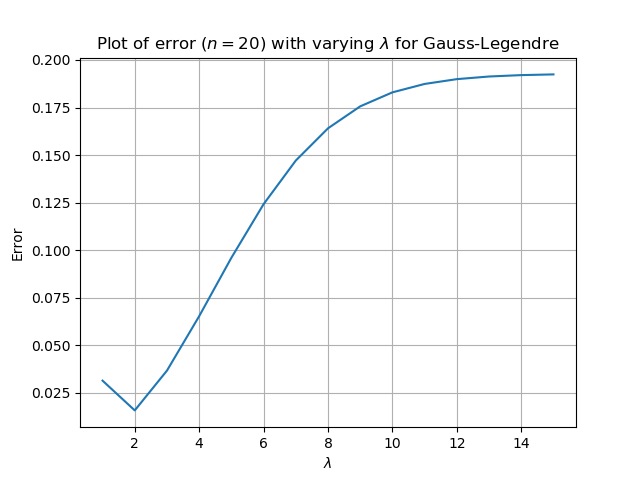
\includegraphics[width = 11cm]{images/error-lambda.png}
  	\caption{The plot of error as a function of $\lambda$ for Gauss-Legendre. }
    \label{fig:lambdapng}
  \end{figure}

  Gauss-Legendre is dependent on $\lambda$, which defines the integration limits. Therefore, it is important to investigate which value of $\lambda$ gives the best approximation of the integral. Figure (\ref{fig:lambdapng}) plots the error as a function of $\lambda$ for Gauss-Legendre. When $\lambda = 2$ the approximation is best. Table (\ref{tab:lambda}) below gives the values of the plot. \\

  \begin{table}[ht]
      \centering
      \caption{Error and time for Gauss-Legendre as a function of $\lambda$ with the set value $n = 20$. }
      \vspace{2mm}
      \label{tab:lambda}
      \begin{tabular}{|c|c|c|c|}
          \hline
          $n$ & $\lambda$ & error & time \\
          \hline \hline
          20 & 1 & 0.0313459 & 3.35521 \\
          20 & 2 & 0.0157005 & 3.32988 \\
          20 & 3 & 0.0366263 & 3.33241 \\
          20 & 4 & 0.0652528 & 3.34317 \\
          20 & 5 & 0.0959769 & 3.33531 \\
          20 & 6 & 0.124165 & 3.33762 \\
          20 & 7 & 0.147104 & 3.33286 \\
          20 & 8 & 0.164053 & 3.34689 \\
          20 & 9 & 0.175608 & 3.33201 \\
          20 & 10 & 0.182966 & 3.33199 \\
          20 & 11 & 0.187388 & 3.3834 \\
          20 & 12 & 0.189917 & 3.41952 \\
          20 & 13 & 0.191303 & 3.33239 \\
          20 & 14 & 0.192035 & 3.32912 \\
          20 & 15 & 0.192409 & 3.47462 \\
          \hline
        \end{tabular} \\
        \hspace{0pt}\\
    \end{table}

\newpage
\clearpage

  \begin{figure}[ht]
    \centering
    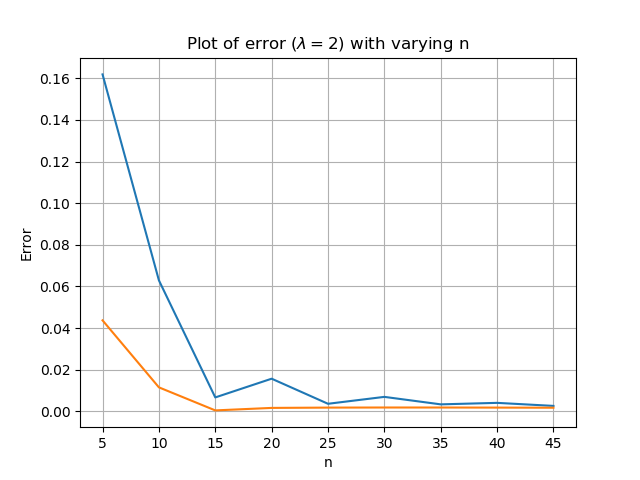
\includegraphics[width = 10cm]{images/error-integrationpoints.png}
    \caption{The plot of error as a function of integrations points $n$ for Gauss-Legendre and Gauss-Laguerre. }
    \label{fig:integrationpointspng}
  \end{figure}

  Figure (\ref{fig:integrationpointspng}) above plots the error as a function of integration points, $n$, for Gauss-Legendre and Gauss-Laguerre. As found above for figure (\ref{fig:lambdapng}) the best approximation of the integral is given when $\lambda = 2$, therefore this is a fixed value in this plot. Table (\ref{tab:error-gauss}) below gives the values of the plot. \\

  \begin{table}[ht]
    \centering
    \caption{Error and execution time for Gauss-Legendre and Gauss-Laguerre.}
    \vspace{2mm}
    \label{tab:error-gauss}
    \begin{tabular}{|c|c|c|c|c|c|}
        \hline
        $n$ & $\lambda$ & Legendre error & Laguerre error & Legendre time & Laguerre time \\
        \hline \hline
        5 & 2 & 0.161836 & 0.0437248 & 0.00082727 & 0.0022169 \\
        10 & 2 & 0.0629315 & 0.0115411 & 0.0520311 & 0.150486 \\
        15 & 2 & 0.00670907 & 0.000476827 & 0.609131 & 1.69456 \\
        20 & 2 & 0.0157005 & 0.00167232 & 3.35013 & 9.3416 \\
        25 & 2 & 0.00365618 & 0.00181852 & 12.8663 & 35.5266 \\
        30 & 2 & 0.00697009 & 0.00186703 & 38.0615 & 105.708 \\
        35 & 2 & 0.00337855 & 0.00186074 & 95.5971 & 264.104 \\
        40 & 2 & 0.00409558 & 0.00181934 & 214.105 & 608.182 \\
        45 & 2 & 0.00263748 & 0.00176034 & 433.725 & 1191.8 \\
        50 & 2 & 0.00281127 & 0.00169433 & 831.449 & 2314.1 \\
        \hline
    \end{tabular} \\
    \hspace{0pt}\\
  \end{table}

\newpage
\clearpage

  \begin{figure}[ht]
    \centering
    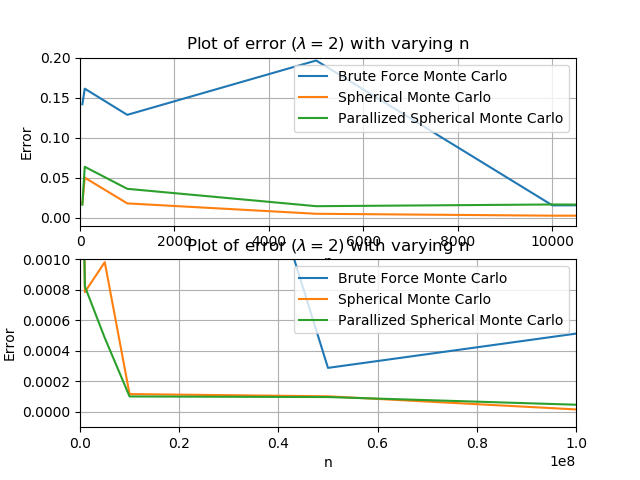
\includegraphics[width = 11cm]{images/error-montecarlo.png}
    \caption{The plot of error as a function of integration points $n$ for brute force Monte Carlo, spherical Monte Carlo, and parallelized spherical Monte Carlo. }
    \label{fig:montecarlopng}
  \end{figure}

  Figure (\ref{fig:montecarlopng}) above plots the error as a function of integration points, $n$, for brute force Monte Carlo, spherical Monte Carlo and parallelized spherical Monte Carlo. As brute force Monte Carlo is dependent on $\lambda$, this is set to be 2 given by figure (\ref{fig:lambdapng}). Table (\ref{tab:error-montecarlo}) below gives the values of the plot. \\

  \begin{table}[ht]
    \centering
    \caption{Error and execution time for brute force Monte Carlo, spherical Monte Carlo, and parallelized spherical Monte Carlo.}
    \vspace{2mm}
    \label{tab:error-montecarlo}
    \begin{tabular}{|c|c|c|c|c|c|c|c|}
        \hline
        $n$ & $\lambda$ & BMC error & SMC error & PSMC error & BMC time & SMC time & PSMC time  \\
        \hline \hline
        50 & 2 & 0.138417 & 0.251552 & 0.131809 & 0.00011814 & 8.7853e-05 & 0.00038 \\
        100 & 2 & 0.157825 & 0.156198 & 0.0071997 & 0.00014777 & 0.0001193 & 0.00037 \\
        500 & 2 & 0.113224 & 0.012164 & 0.00302251 & 0.0003764 & 0.0003822 & 0.00051 \\
        1000 & 2 & 0.079204 & 0.0168798 & 0.022215 & 0.00066215 & 0.0007048 & 0.00098 \\
        5000 & 2 & 0.029304 & 0.011712 & 0.013536 & 0.0029481 & 0.00338986 & 0.002612 \\
        10000 & 2 & 0.0457817 & 0.00027297 & 0.018113 & 0.005808 & 0.006558 & 0.005258 \\
        50000 & 2 & 0.0096648 & 0.0038374 & 0.0012646 & 0.029013 & 0.032508 & 0.025366 \\
        100000 & 2 & 0.024003 & 0.0043587 & 0.00030587 & 0.056982 & 0.067961 & 0.047938 \\
        500000 & 2 & 0.0137398 & 0.0046188 & 0.00356363 & 0.287352 & 0.328019 & 0.18964 \\
        1000000 & 2 & 0.0161491 & 0.00049579 & 0.0005530 & 0.57400 & 0.654257 & 0.354581 \\
        5000000 & 2 & 0.00311977 & 0.00048176 & 0.00026134 & 2.85616 & 3.27695 & 1.82245 \\
        10000000 & 2 & 0.00481115 & 0.00012881 & 2.40583e-05 & 5.70269 & 6.54182 & 3.3623 \\
        50000000 & 2 & 0.00265522 & 9.08138e-05 & 5.988e-05 & 29.7091 & 33.0613 & 16.5097 \\
        100000000 & 2 & 0.00117823 & 0.0001726 & 7.16594e-05 & 58.8054 & 67.2903 & 33.4236 \\
        500000000 & 2 & 6.0793e-05 & 2.5923e-05 & 1.6625e-05 & 415.953 & 448.229 & 208.211 \\
        \hline
    \end{tabular} \\
    \hspace{0pt}\\
  \end{table}

  \newpage
  \clearpage

  \begin{figure}[ht]
    \centering
    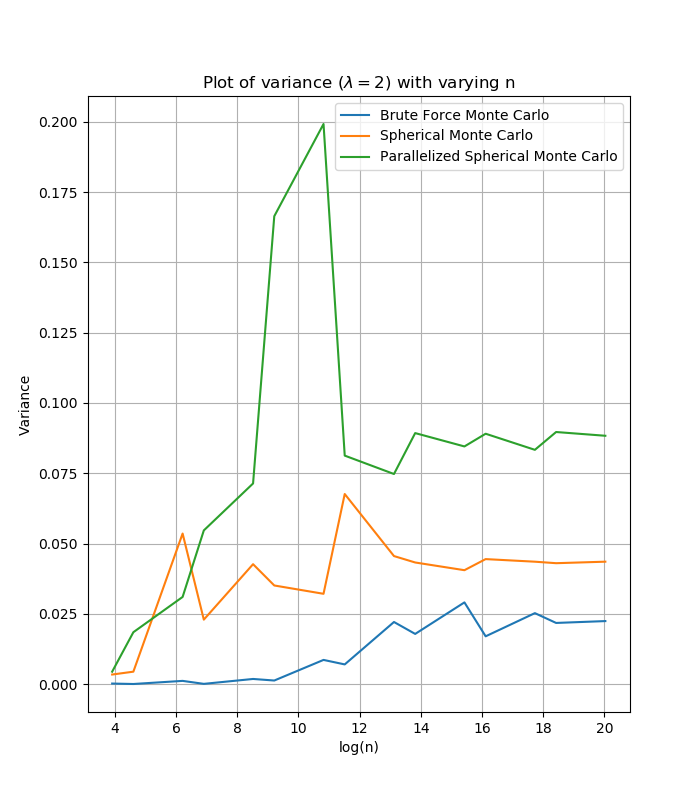
\includegraphics[width = 11cm]{images/variance-montecarlo.png}
    \caption{The plot of variance as a function of the logarithm of integration points $n$ for brute force Monte Carlo, spherical Monte Carlo, and parallelized spherical Monte Carlo. }
    \label{fig:variancemontecarlopng}
  \end{figure}

  Figure (\ref{fig:variancemontecarlopng}) plots the variance of the Monte Carlo methods as a function of the logarithm of the integration points, $n$. The integration points is plotted given by the logarithm of the values because of the large interval of $n$. This way the plot is more condensed, while still illustrating the point of the figure. \\

  \newpage

  Table (\ref{tab:optimalization-montecarlo}) gives the runs of the Monte Carlo methods with different compiler optimalization flags. Since the compiler flags is the variable, the integration points is set to be $n = 5 \cdot 10^8$, to ensure a high accuracy of the approximation to the integral.

  \begin{table}[ht]
    \centering
    \caption{Error and execution time for brute force Monte Carlo, spherical Monte Carlo, and parallelized spherical Monte Carlo when testing different compiler optimalization flags with $\lambda = 2$.}
    \vspace{2mm}
    \label{tab:optimalization-montecarlo}
    \begin{tabular}{|c|c|c|c|c|c|c|c|}
        \hline
        Compiler flag & $n$ & BMC error & SMC error & PSMC error & BMC time & SMC time & PSMC time  \\
        \hline \hline
        none & 500000000 & 6.07925e-05 & 2.59234e-05 & 1.66251e-05 & 415.953 & 448.229 & 208.211 \\
        -O & 500000000 & 0.001144 & 3.8324e-05 & 5.9218e-05 & 140.108 & 170.505 & 75.0108 \\
        -O0 & 500000000 & 9.9830e-05 & 1.5527e-05 & 8.7296e-05 & 368.159 & 429.329 & 197.266 \\
        -O1 & 500000000 & 0.0005797 & 2.9770e-05 & 3.3298e-05 & 206.356 & 231.86 & 113.938 \\
        -O2 & 500000000 & 4.7324e-05 & 4.7423e-05 & 2.5998e-05 & 138.492 & 168.688 & 74.8991 \\
        -O3 & 500000000 & 0.001158 & 0.0001025 & 7.5507e-06 & 141.051 & 160.792 & 71.5184 \\
        \hline
    \end{tabular} \\
    \hspace{0pt}\\
  \end{table}


%--------------- Discussion ---------------------------------------
\vspace{1cm}

\clearpage
\newpage

\section{Discussion} \label{sec:Discussion}

Both Gauss-Legendre and brute force Monte Carlo use $\lambda$ as a parameter for the integration limits. Looking at table (\ref{tab:lambda}) and figure (\ref{fig:lambdapng}) we can see how the accuracy of Gauss-Legendre depends on the value of $\lambda$. We see that the time is more or less constant (as it should be), and that $\lambda=2$ works best. A too small $\lambda$ will give an evaluation of a too small area of the wave-function. A too large $\lambda$ would not give a large improvement, since the wave-function goes to zero after a certain length. In fact, since $\lambda$ increases, the distance between the mesh points will increase, resulting in reduced accuracy.
For Gauss-Legendre, we need about $15$ mesh points to achieve an accuracy of 3 leading digits. For brute force Monte Carlo, this happens at around $n=50000$. This sounds like a lot, but keep in mind that Monte Carlo requires many more points, but by that same token, is much more efficient. \\

Moving from Gauss-Legendre to Gauss-Laguerre, we see an immediate improvement in the numerical accuracy. See figure (\ref{fig:integrationpointspng}) and table (\ref{tab:error-gauss}). However, the method takes more time. The improvement in accuracy is not surprising as Gauss-Laguerre is implemented as an improved Gaussian quadrature. The reason it is more accurate is because Gauss-Laguerre specializes in exponential functions, which our integral is. By changing from a cartesian coordinate system to a spherical one, we can calculate the radial part using Gauss-Laguerre. For this part we also change the limits from $-\lambda \to \lambda$ to $0 \to \infty$. This is great as Laugerre has the limits $0 \to \infty$. The rest of the integral (azimutal and polar parts) are technically still Gauss-Legendre. This explains the increase in time. With pure Gauss-Legendre, we only found the weights once, and reused them. However, with Gauss-Laguerre, we find the weights three times. This is mainly what leads to the increase in time. \\

By looking at table (\ref{tab:error-gauss}) we see that Gaussian quadrature improves greatly by increasing the amount of mesh points, at least for smaller $n$. When we pass about $n=30$ we start getting diminishing returns. The calculation starts taking a very long time, and the improvement in error is not as great as it was for smaller values. \\

After implementing brute force Monte Carlo, we compared it to Gaussian quadrature. It seems the Monte Carlo method is a lot more efficient. This is attributed to the speedy calculation of Monte Carlo. Even though it requires a lot more data points we gain a lot of accuracy by running the same codes for the same amount of time. Looking at table (\ref{tab:error-gauss}) and table (\ref{tab:error-montecarlo}) we see that around $400$ seconds of runtime for the different Gaussian quadratures gives around 3 leading digits of accuracy. The same runtime for brute force Monte Carlo, (BMC), gives 5 leading digits of accuracy. When looking at lower times one can be fooled as Monte Carlo has more or less the same accuracy. However, the Gaussian quadrature methods plateau around 3 digits, whilst BMC keeps improving. \\

Comparing the brute force Monte Carlo method, (BMC), with the spherical Monte Carlo method, (SMC), we can observe a noticeable increase in accuracy. In order to achieve 3 leading digits of accuracy, brute force Monte Carlo needs about $2.90\cdot10^{-2}$ seconds, whilst the spherical Monte Carlo needs around $6.56\cdot10^{-3}$. See table (\ref{tab:error-montecarlo}) and figure (\ref{fig:montecarlopng}). This means a spherical coordinate system indeed is an improvement to Monte Carlo. \\

Monte Carlo is a data-hungry method, and as such, it requires a lot of data points. Looking at table (\ref{tab:error-montecarlo}) we see that it is not great at the same values of $n$ as Gaussian quadrature. At the same time, it is easy to see that Monte Carlo is much faster. Only on values for $n=50000000$ and beyond, Monte Carlo starts struggling. After implementing parallelization the code also sped up by a factor of the machine's available cores (2 in our case). \\

The results show that the parallelized code actually is not better than the non-parallelized spherical Monte Carlo code. This is strange. However, it can be attributed to the fact that the computer running the code only has two cores, meaning there is less of an effect. In addition, there is always the possibility of some mistake in the code. We also divided the element of each sum by $n_{local}$ and took the average of the two cores results, instead of dividing each element in the sum by $n_{total}$.
This could have resulted in a minor loss of precision, but probably not by a lot. As the parallelized spherical Monte Carlo method is about twice as fast, we know that the code is functional. However, it seems there is a loss of numerical precision there. \\

Figures (\ref{fig:timingssmallpng}) and (\ref{fig:timingslargepng}) found in the appendix plots the error as a function of time, and helps to illustrate how the error varies with time for each of the numerical methods in this study. \\

When comparing the different Monte Carlo methods it is interesting to look at how the variance changes. One would think that the variance should decrease when implementing a better method. However, we can see that the variance increases after implementing importance sampling, given by spherical coordinates, when looking at figure (\ref{fig:variancemontecarlopng}). After implementing parallelization, the variance increases even further. This is highly suspect, and after comparing the data, we cannot help but be confused as the error still decreases like $BMC \to SMC \to PSMC$. The reason the variance increases can possibly be attributed to an error in the code. However, this is not that likely as the results still improve. It might be that the variance simply does increase, and that is natural, though we cannot quite make sense of it. \\

Table (\ref{tab:optimalization-montecarlo}) shows the effect of compiler optimalization flags on the Monte Carlo methods for $n = 5 \cdot 10^8$ integration points. Here it is possible to observe that the choice of compiler flags clearly has an effect, mainly the difference between no compiler flag and -O3 exemplifies the huge impact of compiler flags. The row for no compiler flags is taken from table (\ref{tab:error-montecarlo}). When using -O3 compiler flag it is roughly $34 \%$ faster than no compiler flag, which is a huge improvement in execution time. However, the execution time may be faster, but the accuracy of the approximation to the integral is somewhat inferior. While the error of the parallelized spherical Monte Carlo method is better, the errors for brute force Monte Carlo and spherical Monte Carlo is worse, making the compiler flag a bad alternative to no compiler flag. The error for the other compiler flags follows the same trend, where the execution time is faster, but the accuracy of the approximation is worse. Therefore, running the program with no compiler optimalization flag is the better option for best results.


%---------------Conclusion and perspective---------------------------
\vspace{1cm}

\section{Conclusion and perspective} \label{sec:Conclusion}

To conclude, the Monte Carlo integration methods exceeded the Gaussian quadrature methods for both computation time and accuracy. As expected the parallelized spherical Monte Carlo was the fastest method with the highest degree of accuracy. This is mainly because the computation is divided upon all of the machine's available cores, giving it the opportunity to calculate with a lot more data points, or the same amount of data points in a lower amount of time. \\

Seeing as Gaussian quadrature first has to find weights for all points and then calculate the integral, it takes a lot of time. Monte Carlo methods choose random points, do not calculate weights and therefore use less time to calculate. It needs a lot of data points in order to truly shine, but its speed and efficiency turns it into an extraordinarily good method.

%--------------Appendix---------------------------------------------
\vspace{1cm}

\section{Appendix} \label{sec:Appendix}

\subsection{Calculation of Monte Carlo's speed over Gauss-Laguerre} \label{MC>GQ}

We imported the error as function of time for spherical Monte Carlo, SMC, and Gauss-Laguerre into the program Geogebra and did a simple regression analysis. For both data sets, the $f(x) = C x^p$ was the best fit. By extrapolating to $ \varepsilon = 0.001$ we found SMC to intersect at $0.639487186$ and Gauss-Laguerre to intersect at $2284.1372326374$. Dividing Laguerre with SMC, we found SMC to be $3571.82643$ times faster than Gauss-Laguerre. Approximately $3572$ times faster. This seems crazy high, so we have also included the calculation for the actual time for the 1st run where Laugerre and SMC went below $\varepsilon = 0.001$. See below. \\

The 1st time improved spherical Monte Carlo achieved an absolute error below $0.001$ was with $n=10000$. The error was $0.000272967$ and it took $0.00655811$ seconds. The 1st time Gauss-Laguerre achieved an absolute error below $0.001$ was with $n=15$. The error was $0.000476827$ and it took $1.69456$ seconds. \\

Calculation follows: \\

$$\frac{time_{Laguerre}}{time_{SMC}} = \frac{1.69456}{0.00655811} = 258.3915183$$ \\

Spherical Monte Carlo was approximately $258$ times faster than Gauss-Laguerre.\\

\begin{figure}[ht]
    \centering
    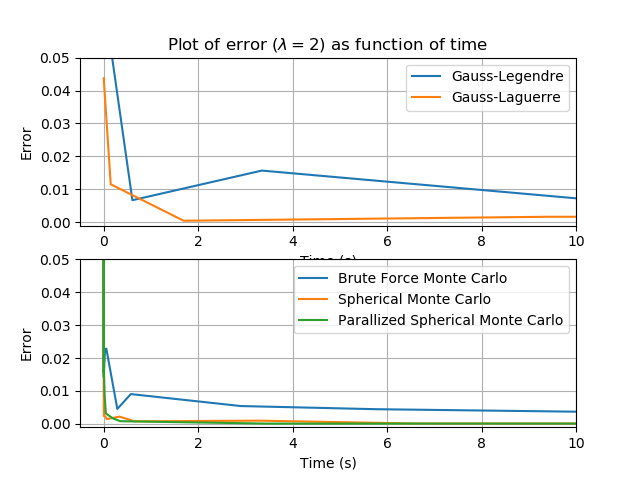
\includegraphics[width = 11cm]{images/method-timings-small.png}
    \caption{The plot of error as a function of time for all the numerical integration methods used in this scientific study. }
    \label{fig:timingssmallpng}
\end{figure}

Figure (\ref{fig:timingslargepng}) does not include all larger data points from our \texttt{.txt}-files. These can be found in table (\ref{tab:error-montecarlo}) for the latter rows. These values can also be found in the file \texttt{montecarlo.txt} on our GitHub, \cite{github}. \\

\vspace{3cm}

\begin{figure}[ht]
    \centering
    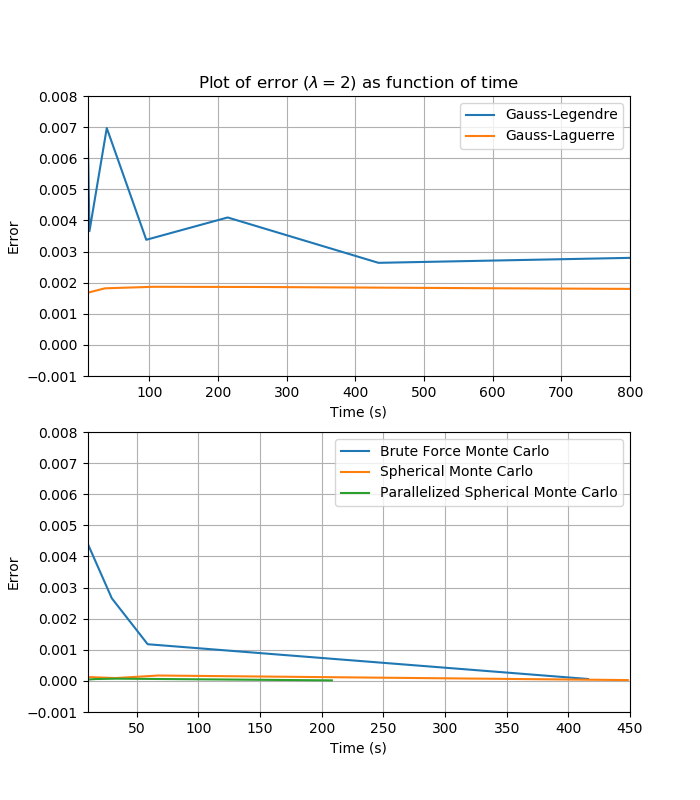
\includegraphics[width = 11cm]{images/method-timings-large.png}
    \caption{This figure is a continuation of the previous figure, (\ref{fig:timingssmallpng}). }
    \label{fig:timingslargepng}
\end{figure}

%\clearpage

%----------------References----------------------------------------

\vspace{1cm}

\section{References} \label{sec:References}

\begin{thebibliography}{}

\bibitem{task}
Morten H. Jensen (2019), \href{https://github.com/CompPhysics/ComputationalPhysics/blob/master/doc/Projects/2019/Project3/pdf/Project3.pdf}{Project 3}, Departement of Physics, University of Oslo, Norway

\bibitem{github}
Erik B. Grammeltvedt, Alexandra Jahr Kolstad, Erlend T. North (2019), \href{https://github.com/Erikbgram/Fys3150}{GitHub}, Students of Departement of Physics, University of Oslo, Norway

\bibitem{lecture_slides}
Morten H. Jensen (2015), \href{https://github.com/CompPhysics/ComputationalPhysics/blob/master/doc/Lectures/lectures2015.pdf}{Lecture slides for FYS3150}, Department of Physics, University of Oslo, Norway

\bibitem{laguerre_polynomial}
Weisstein, Eric W. \href{http://mathworld.wolfram.com/LaguerrePolynomial.html}{"Laguerre Polynomial."}, From MathWorld--A Wolfram Web Resource.


\end{thebibliography}


%----------------Slutten av dokumentet---------------------------------------


%\end{multicols}

\end{document}
